\newpage
\chapter{ANÁLISIS DEL SISTEMA DE INFORMACIÓN}
	\vspace{2cm}	
	\begin{center}
	{\Large \textbf{FASE DE DESARROLLO} \par}
	\end{center}
	\vspace{5cm}
	
	\begin{center}
	\Huge \textbf{ASI}\par
	\end{center}

%\newpage
%\section{ASI 1: DEFINICIÓN DEL SISTEMA}

%\subsection{Determinación del Alcance del Sistema}



\newpage
\section{ASI 2: ESTABLECIMIENTO DE REQUISITOS}
\subsection{Obtención de los Requisitos del Sistema} 

\subsubsection{Requisitos de interfaces externas}

\paragraph*{Interfaces de usuario}
	
	\newlist{myEnumIU}{enumerate}{4}
	\setlist[myEnumIU,1]{label=\textbf{RIU-\arabic*.}}
	\setlist[myEnumIU,2]{label*=\textbf{\arabic*.}}
	\setlist[myEnumIU,3]{label*=\textbf{\arabic*.}}
	\setlist[myEnumIU,4]{label*=\textbf{\arabic*.}}

	\begin{myEnumIU}
		\item El sistema será accesible desde cualquier dispositivo que cuente con conexión a internet y un navegador web.
		\item El sistema estará disponible en diferentes idiomas.
		\begin{myEnumIU}
			\item Español
			\item Inglés
		\end{myEnumIU}
		\item El sistema deberá ser accesible para todos los usuarios a través de los navegadores más comunes.
		\begin{myEnumIU}
			\item Google Chrome
			\item Mozilla Firefox
			\item Microsoft Edge
		\end{myEnumIU}
		\item El usuario podrá utilizar todas las funcionalidades desarrolladas de la aplicación sin inconvenientes.
		\item El usuario no necesitará de conocimientos tecnológicos avanzados.
	\end{myEnumIU}

\paragraph*{Interfaces hardware}
	
	\newlist{myEnumIH}{enumerate}{4}
	\setlist[myEnumIH,1]{label=\textbf{RIH-\arabic*.}}
	\setlist[myEnumIH,2]{label*=\textbf{\arabic*.}}
	\setlist[myEnumIH,3]{label*=\textbf{\arabic*.}}
	\setlist[myEnumIH,4]{label*=\textbf{\arabic*.}}

	\begin{myEnumIH}
		\item El sistema dispondrá de una base de datos para almacenar la información necesaria.
	\end{myEnumIH}

%\paragraph*{Interfaces software}

\paragraph*{Interfaces de comunicaciones}

	\newlist{myEnumIC}{enumerate}{4}
	\setlist[myEnumIC,1]{label=\textbf{RIC-\arabic*.}}
	\setlist[myEnumIC,2]{label*=\textbf{\arabic*.}}
	\setlist[myEnumIC,3]{label*=\textbf{\arabic*.}}
	\setlist[myEnumIC,4]{label*=\textbf{\arabic*.}}

	\begin{myEnumIC}
		\item El sistema contendrá enlaces a diferentes sitios web.
		\item El sistema mostrará por defecto enlaces a los siguientes sitios web.
		\begin{myEnumIC}
			\item Twitter oficial de la Escuela de Ingeniería Informática
			\item Página web de la Escuela de Ingeniería Informática
			\item Página web de la Universidad de Oviedo
		\end{myEnumIC}
	\end{myEnumIC}



\subsubsection{Requisitos funcionales}

\newlist{myEnumerate}{enumerate}{9}
\setlist[myEnumerate,1]{label=\textbf{RF-\arabic*.}}
\setlist[myEnumerate,2]{label*=\textbf{\arabic*.}}
\setlist[myEnumerate,3]{label*=\textbf{\arabic*.}}
\setlist[myEnumerate,4]{label*=\textbf{\arabic*.}}
\setlist[myEnumerate,5]{label*=\textbf{\arabic*.}}
\setlist[myEnumerate,6]{label*=\textbf{\arabic*.}}
\setlist[myEnumerate,7]{label*=\textbf{\arabic*.}}
\setlist[myEnumerate,8]{label*=\textbf{\arabic*.}}
\setlist[myEnumerate,9]{label*=\textbf{\arabic*.}}

\begin{myEnumerate}
\item
\end{myEnumerate}


\subsubsection{Requisitos de rendimiento}
\subsubsection{Requisitos lógicos de BD}
\subsubsection{Requisitos de desarrollo}
\subsubsection{Restricciones de diseño}
\subsubsection{Atributos del sistema}


\subsection{Identificación de Actores del Sistema} 
\subsubsection{Usuario administrador}
Actor que interactúa con el sistema. Es responsable de gestionar el sistema y su mantenimiento. Es el único actor con acceso a la base de datos del sistema y capacidad de modificarla. Debe tener amplios conocimientos sobre el sistema.
\subsubsection{Usuario estándar}
Actor que interactúa con el sistema. Tiene acceso de lectura a toda la aplicación web, exceptuando la parte dedicada al mantenimiento. Solo debe tener un conocimiento básico para navegar por internet.

\subsection{Especificación de Casos de Uso}

\textcolor[rgb]{0.65,0.16,0}{Ejemplo de tabla para especificación de casos de uso}

\begin{table}[htbp]
  \centering
  \caption{Especificación Caso de Uso 1}
    \begin{tabular}{p{20.855em}r}
\cmidrule{1-1}    \rowcolor[rgb]{ .949,  .949,  .949} \multicolumn{1}{p{20.855em}}{\textbf{Nombre del caso de uso}} & \multicolumn{1}{r}{\cellcolor[rgb]{ 1,  1,  1}} \\
\cmidrule{1-1}    \multicolumn{1}{p{20.855em}}{Registro} & \multicolumn{1}{r}{} \\
    \midrule
    \rowcolor[rgb]{ .949,  .949,  .949} \multicolumn{2}{p{31.64em}}{\textbf{Descripción}} \\
    \midrule
    \multicolumn{2}{p{31.64em}}{Un usuario no registrado debe poder registrarse en el sistema mediante su cuenta de Google, lo que hará que automáticamente se inicie sesión en la aplicación.} \\
    \bottomrule
    \end{tabular}%
  \label{espec_caso_uso_1}%
  \vspace{-4mm}
\end{table}%



%\newpage
%\section{ASI 3: IDENTIFICACIÓN DE SUBSISTEMAS DE ANÁLISIS}
%
%\subsection{Descripción de los Subsistemas} 
%%A continuación se describen los subsistemas identificados en el análisis
%%\subsubsection{Vistas}
%%
%%\subsubsection{Modelos}
%%
%%\subsubsection{Bases de datos}
%%
%%\subsubsection{Servidor}
%
%
%\subsection{Descripción de los Interfaces entre Subsistemas}



\newpage
\section{ASI 4: ANÁLISIS DE LOS CASOS DE USO}
\subsection{Caso de Uso 1} 

\begin{table}[H]
  \centering
  \vspace{-5mm}
  \caption{Análisis del Caso de Uso 1}
    \begin{tabular}{p{7.5em}p{24.145em}}
    \toprule
    \rowcolor[rgb]{ .871,  .918,  .965} \multicolumn{2}{p{31.645em}}{\textbf{Consultar periodos (museo)}} \\
    \midrule
    \rowcolor[rgb]{ .906,  .902,  .902} \textbf{Precondiciones} & \cellcolor[rgb]{ 1,  1,  1}- \\
    \midrule
    \rowcolor[rgb]{ .906,  .902,  .902} \textbf{Postcondiciones} & \cellcolor[rgb]{ 1,  1,  1}- \\
    \midrule
    \rowcolor[rgb]{ .906,  .902,  .902} \textbf{Actores} & \cellcolor[rgb]{ 1,  1,  1}Usuario estándar \\
    \midrule
    \rowcolor[rgb]{ .906,  .902,  .902} \textbf{Descripción} & \cellcolor[rgb]{ 1,  1,  1}El usuario accederá a la vista principal del museo y podrá visualizar los periodos existentes. Podrá acceder a los periodos. Podrá acceder a los componentes de los periodos. Podrá realizar una búsqueda.\\
    \midrule
    \rowcolor[rgb]{ .906,  .902,  .902} \textbf{Escenarios          Secundarios} & \cellcolor[rgb]{ 1,  1,  1}  \\
    \bottomrule
    \end{tabular}%
\end{table}%
 
\subsection{Caso de Uso 2}
\begin{table}[H]
  \centering
  \vspace{-5mm}
  \caption{Análisis del Caso de Uso 2}
    \begin{tabular}{p{7.5em}p{24.145em}}
    \toprule
    \rowcolor[rgb]{ .871,  .918,  .965} \multicolumn{2}{p{31.645em}}{\textbf{Consultar componentes (museo)}} \\
    \midrule
    \rowcolor[rgb]{ .906,  .902,  .902} \textbf{Precondiciones} & \cellcolor[rgb]{ 1,  1,  1}- \\
    \midrule
    \rowcolor[rgb]{ .906,  .902,  .902} \textbf{Postcondiciones} & \cellcolor[rgb]{ 1,  1,  1}- \\
    \midrule
    \rowcolor[rgb]{ .906,  .902,  .902} \textbf{Actores} & \cellcolor[rgb]{ 1,  1,  1}Usuario estándar \\
    \midrule
    \rowcolor[rgb]{ .906,  .902,  .902} \textbf{Descripción} & \cellcolor[rgb]{ 1,  1,  1}El usuario accederá a la vista de un periodo y podrá visualizar los componentes pertenecientes al mismo. Podrá acceder a otros periodos. Podrá acceder a los otros componentes de ese periodo. \\
    \midrule
    \rowcolor[rgb]{ .906,  .902,  .902} \textbf{Escenarios          Secundarios} & \cellcolor[rgb]{ 1,  1,  1}  \\
    \bottomrule
    \end{tabular}%
\end{table}%
 
\subsection{Caso de Uso 3}
\begin{table}[H]
  \centering
  \vspace{-5mm}
  \caption{Análisis del Caso de Uso 3}
    \begin{tabular}{p{7.5em}p{24.145em}}
    \toprule
    \rowcolor[rgb]{ .871,  .918,  .965} \multicolumn{2}{p{31.645em}}{\textbf{Iniciar sesión}} \\
    \midrule
    \rowcolor[rgb]{ .906,  .902,  .902} \textbf{Precondiciones} & \cellcolor[rgb]{ 1,  1,  1}El usuario no debe haber iniciado sesión. \\
    \midrule
    \rowcolor[rgb]{ .906,  .902,  .902} \textbf{Postcondiciones} & \cellcolor[rgb]{ 1,  1,  1}- \\
    \midrule
    \rowcolor[rgb]{ .906,  .902,  .902} \textbf{Actores} & \cellcolor[rgb]{ 1,  1,  1}Usuario \\
    \midrule
    \rowcolor[rgb]{ .906,  .902,  .902} \textbf{Descripción} & \cellcolor[rgb]{ 1,  1,  1}El usuario accederá a la página principal de la aplicación de administración e introducirá su email y contraseña para iniciar sesión en el sistema. \\
    \midrule
    \rowcolor[rgb]{ .906,  .902,  .902} \textbf{Escenarios          Secundarios} & \cellcolor[rgb]{ 1,  1,  1} Los datos introducidos no se corresponden con los datos de un usuario con permiso de administrador. Se muestra un error y de nuevo se solicita iniciar sesión. \\
    \bottomrule
    \end{tabular}%
\end{table}%
 
\subsection{Caso de Uso 4}
\begin{table}[H]
  \centering
  \vspace{-5mm}
  \caption{Análisis del Caso de Uso 4}
    \begin{tabular}{p{7.5em}p{24.145em}}
    \toprule
    \rowcolor[rgb]{ .871,  .918,  .965} \multicolumn{2}{p{31.645em}}{\textbf{Consultar periodos (administración)}} \\
    \midrule
    \rowcolor[rgb]{ .906,  .902,  .902} \textbf{Precondiciones} & \cellcolor[rgb]{ 1,  1,  1}El usuario debe haber iniciado sesión. \\
    \midrule
    \rowcolor[rgb]{ .906,  .902,  .902} \textbf{Postcondiciones} & \cellcolor[rgb]{ 1,  1,  1}- \\
    \midrule
    \rowcolor[rgb]{ .906,  .902,  .902} \textbf{Actores} & \cellcolor[rgb]{ 1,  1,  1}Usuario administrador \\
    \midrule
    \rowcolor[rgb]{ .906,  .902,  .902} \textbf{Descripción} & \cellcolor[rgb]{ 1,  1,  1}El usuario accederá al listado de periodos. Podrá acceder a cada uno de ellos. \\
    \midrule
    \rowcolor[rgb]{ .906,  .902,  .902} \textbf{Escenarios          Secundarios} & \cellcolor[rgb]{ 1,  1,  1}Aún no existe ningún periodo en el sistema. Se muestra una tabla vacía. \\
    \bottomrule
    \end{tabular}%
\end{table}
 
\subsection{Caso de Uso 5}
\begin{table}[H]
  \centering
  \vspace{-5mm}
  \caption{Análisis del Caso de Uso 5}
    \begin{tabular}{p{7.5em}p{24.145em}}
    \toprule
    \rowcolor[rgb]{ .871,  .918,  .965} \multicolumn{2}{p{31.645em}}{\textbf{Añadir periodo}} \\
    \midrule
    \rowcolor[rgb]{ .906,  .902,  .902} \textbf{Precondiciones} & \cellcolor[rgb]{ 1,  1,  1}El usuario debe haber iniciado sesión. \\
    \midrule
    \rowcolor[rgb]{ .906,  .902,  .902} \textbf{Postcondiciones} & \cellcolor[rgb]{ 1,  1,  1}El periodo añadido se guardará en la base de datos. \\
    \midrule
    \rowcolor[rgb]{ .906,  .902,  .902} \textbf{Actores} & \cellcolor[rgb]{ 1,  1,  1}Usuario administrador \\
    \midrule
    \rowcolor[rgb]{ .906,  .902,  .902} \textbf{Descripción} & \cellcolor[rgb]{ 1,  1,  1}El usuario accede al formulario para añadir un periodo. Rellena los campos necesarios. Pulsa el botón de guardar. \\
    \midrule
    \rowcolor[rgb]{ .906,  .902,  .902} \textbf{Escenarios          Secundarios} & \cellcolor[rgb]{ 1,  1,  1}- Se pulsa el botón cancelar. El formulario se restablece.\par - Se intenta acceder a otra página de la aplicación sin haber guardado los cambios. Se avisa de la situación y se pide una confirmación para continuar.\par - No se puede añadir el periodo. Se mostrará un error avisando de la situación. \\
    \bottomrule
    \end{tabular}%
\end{table}%
 
\subsection{Caso de Uso 6}
\begin{table}[H]
  \centering
  \vspace{-5mm}
  \caption{Análisis del Caso de Uso 6}
    \begin{tabular}{p{7.5em}p{24.145em}}
    \toprule
    \rowcolor[rgb]{ .871,  .918,  .965} \multicolumn{2}{p{31.645em}}{\textbf{Modificar periodo}} \\
    \midrule
    \rowcolor[rgb]{ .906,  .902,  .902} \textbf{Precondiciones} & \cellcolor[rgb]{ 1,  1,  1}El usuario debe haber iniciado sesión. Debe existir al menos un periodo. \\
    \midrule
    \rowcolor[rgb]{ .906,  .902,  .902} \textbf{Postcondiciones} & \cellcolor[rgb]{ 1,  1,  1}Los cambios realizados al periodo se guardarán en la base de datos. \\
    \midrule
    \rowcolor[rgb]{ .906,  .902,  .902} \textbf{Actores} & \cellcolor[rgb]{ 1,  1,  1}Usuario administrador \\
    \midrule
    \rowcolor[rgb]{ .906,  .902,  .902} \textbf{Descripción} & \cellcolor[rgb]{ 1,  1,  1}El usuario accede al periodo deseado y selecciona la opción de editar. Se mostrará el formulario correspondiente. Se realizan los cambios en el formulario. Pulsa el botón de guardar. \\
    \midrule
    \rowcolor[rgb]{ .906,  .902,  .902} \textbf{Escenarios          Secundarios} & \cellcolor[rgb]{ 1,  1,  1}- Se pulsa el botón cancelar. El formulario se restablece.\par - Se intenta acceder a otra página de la aplicación sin haber guardado los cambios. Se avisa de la situación y se pide una confirmación para continuar.\par - No se puede modificar el periodo. Se mostrará un error avisando de la situación. \\
    \bottomrule
    \end{tabular}%
\end{table}%
 
\subsection{Caso de Uso 7}
\begin{table}[H]
  \centering
  \vspace{-5mm}
  \caption{Análisis del Caso de Uso 7}
    \begin{tabular}{p{7.5em}p{24.145em}}
    \toprule
    \rowcolor[rgb]{ .871,  .918,  .965} \multicolumn{2}{p{31.645em}}{\textbf{Eliminar periodo}} \\
    \midrule
    \rowcolor[rgb]{ .906,  .902,  .902} \textbf{Precondiciones} & \cellcolor[rgb]{ 1,  1,  1}El usuario debe haber iniciado sesión. Debe existir al menos un periodo. \\
    \midrule
    \rowcolor[rgb]{ .906,  .902,  .902} \textbf{Postcondiciones} & \cellcolor[rgb]{ 1,  1,  1}El periodo eliminado y los componentes que pertenecen al mismo se borrarán de la base de datos y dejarán de mostrarse en la aplicación. \\
    \midrule
    \rowcolor[rgb]{ .906,  .902,  .902} \textbf{Actores} & \cellcolor[rgb]{ 1,  1,  1}Usuario administrador \\
    \midrule
    \rowcolor[rgb]{ .906,  .902,  .902} \textbf{Descripción} & \cellcolor[rgb]{ 1,  1,  1}El usuario accede al periodo deseado y selecciona la opción de eliminar. Se pide confirmación para eliminarlo. Se acepta esta confirmación. \\
    \midrule
    \rowcolor[rgb]{ .906,  .902,  .902} \textbf{Escenarios          Secundarios} & \cellcolor[rgb]{ 1,  1,  1}- No se acepta la confirmación para eliminarlo. El periodo y sus componentes permanecen en la base de datos.\par - No se puede eliminar el periodo. Se mostrará un error avisando de la situación. \\
    \bottomrule
    \end{tabular}%
\end{table}%
 
\subsection{Caso de Uso 8}
\begin{table}[H]
  \centering
  \vspace{-5mm}
  \caption{Análisis del Caso de Uso 8}
    \begin{tabular}{p{7.5em}p{24.145em}}
    \toprule
    \rowcolor[rgb]{ .871,  .918,  .965} \multicolumn{2}{p{31.645em}}{\textbf{Consultar componentes (administración)}} \\
    \midrule
    \rowcolor[rgb]{ .906,  .902,  .902} \textbf{Precondiciones} & \cellcolor[rgb]{ 1,  1,  1}El usuario debe haber iniciado sesión. Debe existir al menos un periodo. \\
    \midrule
    \rowcolor[rgb]{ .906,  .902,  .902} \textbf{Postcondiciones} & \cellcolor[rgb]{ 1,  1,  1}- \\
    \midrule
    \rowcolor[rgb]{ .906,  .902,  .902} \textbf{Actores} & \cellcolor[rgb]{ 1,  1,  1}Usuario administrador \\
    \midrule
    \rowcolor[rgb]{ .906,  .902,  .902} \textbf{Descripción} & \cellcolor[rgb]{ 1,  1,  1}El usuario accederá a un periodo existente y visualizará los componentes pertenecientes a este. Podrá acceder a cada uno de ellos. \\
    \midrule
    \rowcolor[rgb]{ .906,  .902,  .902} \textbf{Escenarios          Secundarios} & \cellcolor[rgb]{ 1,  1,  1}Aún no existen componentes para el periodo que se consulta. Se mostrará una tabla vacía. \\
    \bottomrule
    \end{tabular}%
\end{table}%
 
\subsection{Caso de Uso 9}
\begin{table}[H]
  \centering
  \vspace{-5mm}
  \caption{Análisis del Caso de Uso 9}
    \begin{tabular}{p{7.5em}p{24.145em}}
    \toprule
    \rowcolor[rgb]{ .871,  .918,  .965} \multicolumn{2}{p{31.645em}}{\textbf{Añadir componente}} \\
    \midrule
    \rowcolor[rgb]{ .906,  .902,  .902} \textbf{Precondiciones} & \cellcolor[rgb]{ 1,  1,  1}El usuario debe haber iniciado sesión. Debe existir al menos un periodo. \\
    \midrule
    \rowcolor[rgb]{ .906,  .902,  .902} \textbf{Postcondiciones} & \cellcolor[rgb]{ 1,  1,  1}El componente añadido se guardará en la base de datos y se asociará al periodo correspondiente. \\
    \midrule
    \rowcolor[rgb]{ .906,  .902,  .902} \textbf{Actores} & \cellcolor[rgb]{ 1,  1,  1}Usuario administrador \\
    \midrule
    \rowcolor[rgb]{ .906,  .902,  .902} \textbf{Descripción} & \cellcolor[rgb]{ 1,  1,  1}El usuario accede al formulario para añadir un componente. Rellena los campos necesarios. Pulsa el botón de guardar. \\
    \midrule
    \rowcolor[rgb]{ .906,  .902,  .902} \textbf{Escenarios          Secundarios} & \cellcolor[rgb]{ 1,  1,  1}- Se pulsa el botón cancelar. El formulario se restablece.\par - Se intenta acceder a otra página de la aplicación sin haber guardado los cambios. Se avisa de la situación y se pide una confirmación para continuar.\par - No se puede añadir el componente. Se mostrará un error avisando de la situación.  \\
    \bottomrule
    \end{tabular}%
\end{table}%
 
\subsection{Caso de Uso 10}
\begin{table}[H]
  \centering
  \vspace{-5mm}
  \caption{Análisis del Caso de Uso 10}
    \begin{tabular}{p{7.5em}p{24.145em}}
    \toprule
    \rowcolor[rgb]{ .871,  .918,  .965} \multicolumn{2}{p{31.645em}}{\textbf{Modificar componente}} \\
    \midrule
    \rowcolor[rgb]{ .906,  .902,  .902} \textbf{Precondiciones} & \cellcolor[rgb]{ 1,  1,  1}El usuario debe haber iniciado sesión. Debe existir al menos un componente. \\
    \midrule
    \rowcolor[rgb]{ .906,  .902,  .902} \textbf{Postcondiciones} & \cellcolor[rgb]{ 1,  1,  1}Los cambios realizados en el componente se guardarán en la base de datos. \\
    \midrule
    \rowcolor[rgb]{ .906,  .902,  .902} \textbf{Actores} & \cellcolor[rgb]{ 1,  1,  1}Usuario administrador \\
    \midrule
    \rowcolor[rgb]{ .906,  .902,  .902} \textbf{Descripción} & \cellcolor[rgb]{ 1,  1,  1}El usuario accede al componente deseado y selecciona la opción de editar. Se mostrará el formulario correspondiente. Se realizan los cambios en el formulario. Pulsa el botón de guardar. \\
    \midrule
    \rowcolor[rgb]{ .906,  .902,  .902} \textbf{Escenarios          Secundarios} & \cellcolor[rgb]{ 1,  1,  1}- Se pulsa el botón cancelar. El formulario se restablece.\par - Se intenta acceder a otra página de la aplicación sin haber guardado los cambios. Se avisa de la situación y se pide una confirmación para continuar.\par - No se puede modificar el componente. Se mostrará un error avisando de la situación.  \\
    \bottomrule
    \end{tabular}%
\end{table}
 
\subsection{Caso de Uso 11}
\begin{table}[H]
  \centering
  \vspace{-5mm}
  \caption{Análisis del Caso de Uso 11}
    \begin{tabular}{p{7.5em}p{24.145em}}
    \toprule
    \rowcolor[rgb]{ .871,  .918,  .965} \multicolumn{2}{p{31.645em}}{\textbf{Eliminar componente}} \\
    \midrule
    \rowcolor[rgb]{ .906,  .902,  .902} \textbf{Precondiciones} & \cellcolor[rgb]{ 1,  1,  1}El usuario debe haber iniciado sesión. Debe existir al menos un componente. \\
    \midrule
    \rowcolor[rgb]{ .906,  .902,  .902} \textbf{Postcondiciones} & \cellcolor[rgb]{ 1,  1,  1}El componente eliminado  se borrará de la base de datos y dejará de mostrarse en la aplicación. \\
    \midrule
    \rowcolor[rgb]{ .906,  .902,  .902} \textbf{Actores} & \cellcolor[rgb]{ 1,  1,  1}Usuario administrador \\
    \midrule
    \rowcolor[rgb]{ .906,  .902,  .902} \textbf{Descripción} & \cellcolor[rgb]{ 1,  1,  1}El usuario accede al componente deseado y selecciona la opción de eliminar. Se pide confirmación para eliminarlo. Se acepta esta confirmación.  \\
    \midrule
    \rowcolor[rgb]{ .906,  .902,  .902} \textbf{Escenarios          Secundarios} & \cellcolor[rgb]{ 1,  1,  1}- No se acepta la confirmación para eliminarlo. El componente permanece en la base de datos.\par - No se puede eliminar el componente. Se mostrará un error avisando de la situación.  \\
    \bottomrule
    \end{tabular}%
\end{table}%


\newpage
\section{ASI 5: ANÁLISIS DE CLASES}

\subsection{Diagrama de Clases} 
\subsubsection{Museo}
\begin{figure}[H]
\centering
\centerline{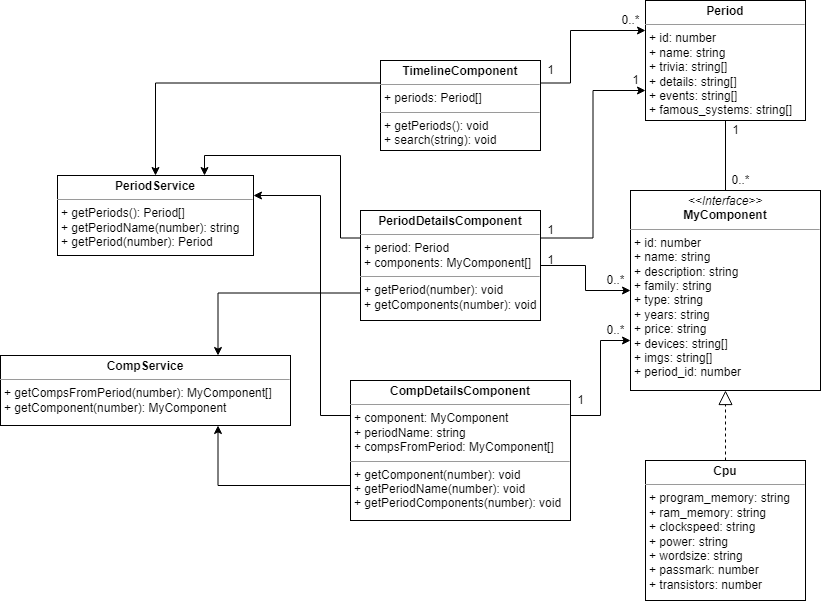
\includegraphics[scale=0.5]{asi-clases-museo}}
\caption{Análisis de clases: diagrama de clases del museo}
\end{figure}
\subsubsection{Administración del museo}
\begin{figure}[H]
\centering
\centerline{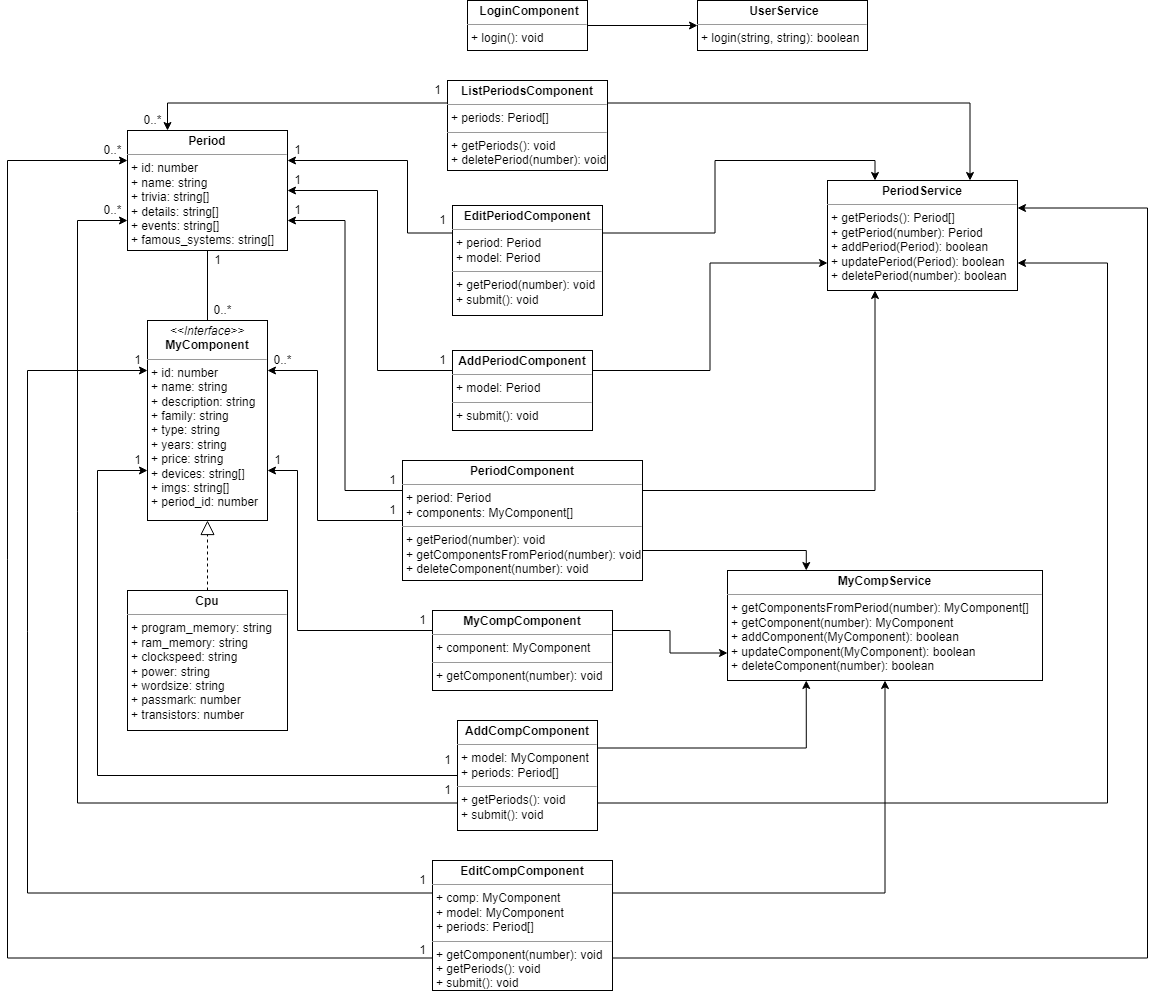
\includegraphics[scale=0.5]{asi-clases-admin}}
\caption{Análisis de clases: diagrama de clases de la administración}
\end{figure}

\subsection{Descripción de las Clases}
\textit{Period}, \textit{MyComponent} y \textit{Cpu} son iguales en el proyecto del museo y en el de la administración, por lo tanto se describen una única vez a continuación:

\begin{table}[H]
\vspace{-4mm}
  \centering
  \caption{Descripción de la clase Period}
    \begin{tabular}{p{8.645em}p{5em}p{15.5em}}
    \toprule
    \rowcolor[rgb]{ .851,  .886,  .953} \multicolumn{3}{p{31.285em}}{\textbf{Periodo}} \\ \midrule
    \rowcolor[rgb]{ .949,  .949,  .949} \multicolumn{3}{p{31.285em}}{\textbf{Descripción}} \\ \midrule
    \multicolumn{3}{p{31.285em}}{Clase que modela un periodo.} \\ \midrule
    \rowcolor[rgb]{ .906,  .902,  .902} \multicolumn{3}{p{31.285em}}{\textbf{Atributos propuestos}} \\ \midrule
    \textbf{id} & number & Identificador del periodo\\
    \textbf{name} & string & Nombre del periodo \\ 
    \textbf{trivia} & string[] & Curiosidades del periodo \\
    \textbf{details} & string[] & Detalles del periodo \\
    \textbf{events} & string[] & Eventos ocurridos durante este periodo \\
    \textbf{famous\_systems} & string[] & Sistemas famosos que llevaban componentes pertenecientes al periodo \\ \midrule
    \rowcolor[rgb]{ .906,  .902,  .902} \multicolumn{3}{p{31.285em}}{\textbf{Métodos propuestos}} \\ \midrule
    \multicolumn{3}{p{31.285em}}{-} \\ \bottomrule
    \end{tabular}%
\end{table}%

\begin{table}[H]
\vspace{-4mm}
  \centering
  \caption{Descripción de la interfaz MyComponent }
    \begin{tabular}{p{8.645em}p{5em}p{15.5em}}
    \toprule
    \rowcolor[rgb]{ .851,  .886,  .953} \multicolumn{3}{p{31.285em}}{\textbf{MyComponent}} \\ \midrule
    \rowcolor[rgb]{ .949,  .949,  .949} \multicolumn{3}{p{31.285em}}{\textbf{Descripción}} \\ \midrule
    \multicolumn{3}{p{31.285em}}{Interfaz que modela los atributos genéricos de un componente.} \\ \midrule
    \rowcolor[rgb]{ .906,  .902,  .902} \multicolumn{3}{p{31.285em}}{\textbf{Atributos propuestos}} \\ \midrule
    \textbf{id} & number & Identificador del componente\\
    \textbf{name} & string & Nombre del componente \\ 
    \textbf{description} & string & Descripción del componente \\
    \textbf{family} & string & Familia a la que pertenece \\
    \textbf{type} & string & Tipo de componente (CPU, genérico...) \\
    \textbf{years} & string & Rango de años en los que se utilizó \\
    \textbf{price} & string & Precio de venta del componente \\
    \textbf{devices} & string[] & Tipo de dispositivos en los que se usaba el componente (portátiles o de escritorio) \\
    \textbf{imgs} & string[] & Nombres de las imágenes del componente \\
    \textbf{period\_id} & number & Identificador del periodo al que pertenece el componente \\ \midrule
    \rowcolor[rgb]{ .906,  .902,  .902} \multicolumn{3}{p{31.285em}}{\textbf{Métodos propuestos}} \\ \midrule
    \multicolumn{3}{p{31.285em}}{-} \\ \bottomrule
    \end{tabular}%
\end{table}%

\begin{table}[H]
\vspace{-4mm}
  \centering
  \caption{Descripción de la clase Cpu}
    \begin{tabular}{p{8.645em}p{5em}p{15.5em}}
    \toprule
    \rowcolor[rgb]{ .851,  .886,  .953} \multicolumn{3}{p{31.285em}}{\textbf{Cpu}} \\ \midrule
    \rowcolor[rgb]{ .949,  .949,  .949} \multicolumn{3}{p{31.285em}}{\textbf{Descripción}} \\ \midrule
    \multicolumn{3}{p{31.285em}}{Clase que implementa la interfaz MyComponent. Modela una CPU, con sus atributos específicos correspondientes. } \\ \midrule
    \rowcolor[rgb]{ .906,  .902,  .902} \multicolumn{3}{p{31.285em}}{\textbf{Atributos propuestos}} \\ \midrule
    \textbf{program\_memory} & string & Memoria ROM de la CPU\\
    \textbf{ram\_memory} & string & Memoria RAM de la CPU\\
    \textbf{clockspeed} & string & Velocidad de reloj de la CPU\\ 
    \textbf{power} & string & Potencia de la CPU\\
    \textbf{wordsize} & string & Tamaño de palabra de la CPU\\
    \textbf{passmark} & number & Passmark de la CPU\\
    \textbf{transistors} & number & Número de transistores de la CPU\\ \midrule
    \rowcolor[rgb]{ .906,  .902,  .902} \multicolumn{3}{p{31.285em}}{\textbf{Métodos propuestos}} \\ \midrule
    \multicolumn{3}{p{31.285em}}{-} \\ \bottomrule
    \end{tabular}%
\end{table}%

\subsubsection{Museo}

\begin{table}[H]
\vspace{-4mm}
  \centering
  \caption{Descripción de la clase PeriodService (museo)}
    \begin{tabular}{p{8.645em}p{5em}p{15.5em}}
    \toprule
    \rowcolor[rgb]{ .851,  .886,  .953} \multicolumn{3}{p{31.285em}}{\textbf{PeriodService}} \\ \midrule
    \rowcolor[rgb]{ .949,  .949,  .949} \multicolumn{3}{p{31.285em}}{\textbf{Descripción}} \\ \midrule
    \multicolumn{3}{p{31.285em}}{Servicio que conecta con el back-end de la aplicación para realizar las operaciones relacionadas con los periodos.} \\ \midrule
    \rowcolor[rgb]{ .906,  .902,  .902} \multicolumn{3}{p{31.285em}}{\textbf{Atributos propuestos}} \\ \midrule
    \multicolumn{3}{p{31.285em}}{-} \\ \midrule
    \rowcolor[rgb]{ .906,  .902,  .902} \multicolumn{3}{p{31.285em}}{\textbf{Métodos propuestos}} \\ \midrule
    \textbf{getPeriods} & \multicolumn{2}{p{22.64em}}{Devuelve todos los periodos existentes.} \\ 
    \textbf{getPeriodName} & \multicolumn{2}{p{22.64em}}{Devuelve el nombre del periodo correspondiente al identificador pasado por parámetro.} \\ 
    \textbf{getPeriod} & \multicolumn{2}{p{22.64em}}{Devuelve el periodo cuyo identificador se pasa como parámetro.} \\ \bottomrule
    \end{tabular}%
\end{table}%

\begin{table}[H]
\vspace{-4mm}
  \centering
  \caption{Descripción de la clase CompService (museo)}
    \begin{tabular}{p{10em}p{5em}p{14.5em}}
    \toprule
    \rowcolor[rgb]{ .851,  .886,  .953} \multicolumn{3}{p{31.285em}}{\textbf{CompService}} \\ \midrule
    \rowcolor[rgb]{ .949,  .949,  .949} \multicolumn{3}{p{31.285em}}{\textbf{Descripción}} \\ \midrule
    \multicolumn{3}{p{31.285em}}{Servicio que conecta con el back-end de la aplicación para realizar las operaciones relacionadas con los componentes.} \\ \midrule
    \rowcolor[rgb]{ .906,  .902,  .902} \multicolumn{3}{p{31.285em}}{\textbf{Atributos propuestos}} \\ \midrule
    \multicolumn{3}{p{31.285em}}{-} \\ \midrule
    \rowcolor[rgb]{ .906,  .902,  .902} \multicolumn{3}{p{31.285em}}{\textbf{Métodos propuestos}} \\ \midrule
    \textbf{getCompsFromPeriod} & \multicolumn{2}{p{19.64em}}{Devuelve los componentes pertenecientes al periodo cuyo identificador se pasa como parámetro.} \\ 
    \textbf{getComponent} & \multicolumn{2}{p{19.64em}}{Devuelve el componente cuyo identificador se pasa como parámetro.} \\ \bottomrule
    \end{tabular}%
\end{table}%

\begin{table}[H]
\vspace{-4mm}
  \centering
  \caption{Descripción de la clase TimelineComponent}
    \begin{tabular}{p{8.645em}p{5em}p{15.5em}}
    \toprule
    \rowcolor[rgb]{ .851,  .886,  .953} \multicolumn{3}{p{31.285em}}{\textbf{TimelineComponent}} \\ \midrule
    \rowcolor[rgb]{ .949,  .949,  .949} \multicolumn{3}{p{31.285em}}{\textbf{Descripción}} \\ \midrule
    \multicolumn{3}{p{31.285em}}{Clase asociada a la vista \ref{iu:timeline}.} \\ \midrule
    \rowcolor[rgb]{ .906,  .902,  .902} \multicolumn{3}{p{31.285em}}{\textbf{Atributos propuestos}} \\ \midrule
    \textbf{periods} & Period[] & Listado de todos los periodos existentes. \\ \midrule
    \rowcolor[rgb]{ .906,  .902,  .902} \multicolumn{3}{p{31.285em}}{\textbf{Métodos propuestos}} \\ \midrule
    \textbf{getPeriods} & \multicolumn{2}{p{22.64em}}{Obtiene los periodos y los asigna a \textit{periods}.} \\ 
    \textbf{search} & \multicolumn{2}{p{22.64em}}{Filtra los periodos según el texto introducido en la búsqueda.} \\ \bottomrule
    \end{tabular}%
\end{table}%

\begin{table}[H]
\vspace{-4mm}
  \centering
  \caption{Descripción de la clase PeriodDetailsComponent}
    \begin{tabular}{p{8.645em}p{7em}p{13.5em}}
    \toprule
    \rowcolor[rgb]{ .851,  .886,  .953} \multicolumn{3}{p{31.285em}}{\textbf{PeriodDetailsComponent}} \\ \midrule
    \rowcolor[rgb]{ .949,  .949,  .949} \multicolumn{3}{p{31.285em}}{\textbf{Descripción}} \\ \midrule
    \multicolumn{3}{p{31.285em}}{Clase asociada a la vista \ref{iu:period-details}.} \\ \midrule
    \rowcolor[rgb]{ .906,  .902,  .902} \multicolumn{3}{p{31.285em}}{\textbf{Atributos propuestos}} \\ \midrule
    \textbf{period} & Period & Periodo del que se muestran los detalles. \\ 
    \textbf{components} & MyComponent[] & Componentes pertenecientes al periodo. \\ \midrule
    \rowcolor[rgb]{ .906,  .902,  .902} \multicolumn{3}{p{31.285em}}{\textbf{Métodos propuestos}} \\ \midrule
    \textbf{getPeriod} & \multicolumn{2}{p{22.64em}}{Obtiene el periodo y lo asigna a \textit{period}.} \\ 
    \textbf{getComponents} & \multicolumn{2}{p{22.64em}}{Obtiene los componentes del periodo y los asigna a \textit{components}.} \\ \bottomrule
    \end{tabular}%
\end{table}%

\begin{table}[H]
\vspace{-4mm}
  \centering
  \caption{Descripción de la clase CompDetailsComponent}
    \begin{tabular}{p{8.645em}p{7em}p{13.5em}}
    \toprule
    \rowcolor[rgb]{ .851,  .886,  .953} \multicolumn{3}{p{31.285em}}{\textbf{CompDetailsComponent}} \\ \midrule
    \rowcolor[rgb]{ .949,  .949,  .949} \multicolumn{3}{p{31.285em}}{\textbf{Descripción}} \\ \midrule
    \multicolumn{3}{p{31.285em}}{Clase asociada a la vista \ref{iu:comp-details}.} \\ \midrule
    \rowcolor[rgb]{ .906,  .902,  .902} \multicolumn{3}{p{31.285em}}{\textbf{Atributos propuestos}} \\ \midrule
    \textbf{component} & MyComponent & Componente del que se muestran los detalles. \\ 
    \textbf{periodName} & string & Nombre del periodo al que pertenece el componente. \\ 
    \textbf{components} & MyComponent[] & Otros componentes pertenecientes al periodo. \\ \midrule
    \rowcolor[rgb]{ .906,  .902,  .902} \multicolumn{3}{p{31.285em}}{\textbf{Métodos propuestos}} \\ \midrule
    \multicolumn{1}{p{10.2em}}{\textbf{getComponent}} & \multicolumn{2}{p{19.64em}}{Obtiene el componente y lo asigna a \textit{component}.} \\ 
    \multicolumn{1}{p{10.2em}}{\textbf{getPeriodName}} & \multicolumn{2}{p{19.64em}}{Obtiene el nombre del periodo y lo asigna a \textit{periodName}.} \\ 
    \multicolumn{1}{p{10.2em}}{\textbf{getPeriodComponents}} & \multicolumn{2}{p{19.64em}}{Obtiene los componentes del periodo y los asigna a \textit{components}.} \\ \bottomrule
    \end{tabular}%
\end{table}%


\subsubsection{Administración del museo}

\begin{table}[H]
\vspace{-4mm}
  \centering
  \caption{Descripción de la clase UserService }
    \begin{tabular}{p{8.645em}p{5em}p{15.5em}}
    \toprule
    \rowcolor[rgb]{ .851,  .886,  .953} \multicolumn{3}{p{31.285em}}{\textbf{UserService}} \\ \midrule
    \rowcolor[rgb]{ .949,  .949,  .949} \multicolumn{3}{p{31.285em}}{\textbf{Descripción}} \\ \midrule
    \multicolumn{3}{p{31.285em}}{Servicio que conecta con el back-end de la aplicación para realizar las operaciones relacionadas con el usuario administrador.} \\ \midrule
    \rowcolor[rgb]{ .906,  .902,  .902} \multicolumn{3}{p{31.285em}}{\textbf{Atributos propuestos}} \\ \midrule
    \multicolumn{3}{p{31.285em}}{-} \\ \midrule
    \rowcolor[rgb]{ .906,  .902,  .902} \multicolumn{3}{p{31.285em}}{\textbf{Métodos propuestos}} \\ \midrule
    \textbf{login} & \multicolumn{2}{p{22.64em}}{Comprueba si el usuario y la contraseña introducidos se corresponden con los existentes en la base de datos.} \\ \bottomrule
    \end{tabular}%
\end{table}%

\begin{table}[H]
\vspace{-4mm}
  \centering
  \caption{Descripción de la clase PeriodService (administración)}
    \begin{tabular}{p{8.645em}p{5em}p{15.5em}}
    \toprule
    \rowcolor[rgb]{ .851,  .886,  .953} \multicolumn{3}{p{31.285em}}{\textbf{PeriodService}} \\ \midrule
    \rowcolor[rgb]{ .949,  .949,  .949} \multicolumn{3}{p{31.285em}}{\textbf{Descripción}} \\ \midrule
    \multicolumn{3}{p{31.285em}}{Servicio que conecta con el back-end de la aplicación para realizar las operaciones relacionadas con los periodos.} \\ \midrule
    \rowcolor[rgb]{ .906,  .902,  .902} \multicolumn{3}{p{31.285em}}{\textbf{Atributos propuestos}} \\ \midrule
    \multicolumn{3}{p{31.285em}}{-} \\ \midrule
    \rowcolor[rgb]{ .906,  .902,  .902} \multicolumn{3}{p{31.285em}}{\textbf{Métodos propuestos}} \\ \midrule
    \textbf{getPeriods} & \multicolumn{2}{p{22.64em}}{Devuelve todos los periodos existentes.} \\ 
    \textbf{getPeriod} & \multicolumn{2}{p{22.64em}}{Devuelve el periodo cuyo identificador se pasa como parámetro.} \\ 
    \textbf{addPeriod} & \multicolumn{2}{p{22.64em}}{Añade el periodo pasado como parámetro a la base de datos.} \\ 
    \textbf{updatePeriod} & \multicolumn{2}{p{22.64em}}{Actualiza el periodo pasado como parámetro en la base de datos.} \\ 
    \textbf{getPeriod} & \multicolumn{2}{p{22.64em}}{Elimina de la base de datos el periodo cuyo identificador se pasa como parámetro.} \\ \bottomrule
    \end{tabular}%
\end{table}%

\begin{table}[H]
\vspace{-4mm}
  \centering
  \caption{Descripción de la clase CompService (administración)}
    \begin{tabular}{p{10em}p{5em}p{14.5em}}
    \toprule
    \rowcolor[rgb]{ .851,  .886,  .953} \multicolumn{3}{p{31.285em}}{\textbf{CompService}} \\ \midrule
    \rowcolor[rgb]{ .949,  .949,  .949} \multicolumn{3}{p{31.285em}}{\textbf{Descripción}} \\ \midrule
    \multicolumn{3}{p{31.285em}}{Servicio que conecta con el back-end de la aplicación para realizar las operaciones relacionadas con los componentes.} \\ \midrule
    \rowcolor[rgb]{ .906,  .902,  .902} \multicolumn{3}{p{31.285em}}{\textbf{Atributos propuestos}} \\ \midrule
    \multicolumn{3}{p{31.285em}}{-} \\ \midrule
    \rowcolor[rgb]{ .906,  .902,  .902} \multicolumn{3}{p{31.285em}}{\textbf{Métodos propuestos}} \\ \midrule
    \textbf{getCompsFromPeriod} & \multicolumn{2}{p{19.64em}}{Devuelve los componentes pertenecientes al periodo cuyo identificador se pasa como parámetro.} \\ 
    \textbf{getComponent} & \multicolumn{2}{p{19.64em}}{Devuelve el componente cuyo identificador se pasa como parámetro.} \\ 
    \textbf{addComponent} & \multicolumn{2}{p{19.64em}}{Añade el componente pasado como parámetro a la base de datos.} \\ 
    \textbf{updateComponent} & \multicolumn{2}{p{19.64em}}{Actualiza el componente pasado como parámetro en la base de datos.} \\ 
    \textbf{getComponent} & \multicolumn{2}{p{19.64em}}{Elimina de la base de datos el componente cuyo identificador se pasa como parámetro.} \\ \bottomrule
    \end{tabular}%
\end{table}%

\begin{table}[H]
\vspace{-4mm}
  \centering
  \caption{Descripción de la clase LoginComponent}
    \begin{tabular}{p{8.645em}p{5em}p{15.5em}}
    \toprule
    \rowcolor[rgb]{ .851,  .886,  .953} \multicolumn{3}{p{31.285em}}{\textbf{LoginComponent}} \\ \midrule
    \rowcolor[rgb]{ .949,  .949,  .949} \multicolumn{3}{p{31.285em}}{\textbf{Descripción}} \\ \midrule
    \multicolumn{3}{p{31.285em}}{Clase asociada a la vista \ref{iu:login}.} \\ \midrule
    \rowcolor[rgb]{ .906,  .902,  .902} \multicolumn{3}{p{31.285em}}{\textbf{Atributos propuestos}} \\ \midrule
    \multicolumn{3}{p{31.285em}}{-} \\ \midrule
    \rowcolor[rgb]{ .906,  .902,  .902} \multicolumn{3}{p{31.285em}}{\textbf{Métodos propuestos}} \\ \midrule
    \textbf{login} & \multicolumn{2}{p{22.64em}}{Comprueba los datos introducidos para iniciar sesión.} \\ \bottomrule
    \end{tabular}%
\end{table}%

\begin{table}[H]
\vspace{-4mm}
  \centering
  \caption{Descripción de la clase ListPeriodsComponent}
    \begin{tabular}{p{8.645em}p{5em}p{15.5em}}
    \toprule
    \rowcolor[rgb]{ .851,  .886,  .953} \multicolumn{3}{p{31.285em}}{\textbf{ListPeriodsComponent}} \\ \midrule
    \rowcolor[rgb]{ .949,  .949,  .949} \multicolumn{3}{p{31.285em}}{\textbf{Descripción}} \\ \midrule
    \multicolumn{3}{p{31.285em}}{Clase asociada a la vista \ref{iu:list-periods}.} \\ \midrule
    \rowcolor[rgb]{ .906,  .902,  .902} \multicolumn{3}{p{31.285em}}{\textbf{Atributos propuestos}} \\ \midrule
    \textbf{periods} & Period[] & Listado de todos los periodos existentes. \\ \midrule
    \rowcolor[rgb]{ .906,  .902,  .902} \multicolumn{3}{p{31.285em}}{\textbf{Métodos propuestos}} \\ \midrule
    \textbf{getPeriods} & \multicolumn{2}{p{22.64em}}{Obtiene los periodos y los asigna a \textit{periods}.} \\ 
    \textbf{deletePeriod} & \multicolumn{2}{p{22.64em}}{Elimina el periodo seleccionado.} \\ \bottomrule
    \end{tabular}%
\end{table}%

\begin{table}[H]
\vspace{-4mm}
  \centering
  \caption{Descripción de la clase PeriodComponent}
    \begin{tabular}{p{8.645em}p{7em}p{13.5em}}
    \toprule
    \rowcolor[rgb]{ .851,  .886,  .953} \multicolumn{3}{p{31.285em}}{\textbf{PeriodComponent}} \\ \midrule
    \rowcolor[rgb]{ .949,  .949,  .949} \multicolumn{3}{p{31.285em}}{\textbf{Descripción}} \\ \midrule
    \multicolumn{3}{p{31.285em}}{Clase asociada a la vista \ref{iu:period}.} \\ \midrule
    \rowcolor[rgb]{ .906,  .902,  .902} \multicolumn{3}{p{31.285em}}{\textbf{Atributos propuestos}} \\ \midrule
    \multicolumn{1}{p{8.645em}}{\textbf{period}} & Period & Periodo del que se muestran los detalles. \\ 
    \multicolumn{1}{p{8.645em}}{\textbf{components}} & MyComponent[] & Componentes pertenecientes al periodo. \\ \midrule
    \rowcolor[rgb]{ .906,  .902,  .902} \multicolumn{3}{p{31.285em}}{\textbf{Métodos propuestos}} \\ \midrule
    \multicolumn{1}{p{13.2em}}{\textbf{getPeriod}} & \multicolumn{2}{p{16.64em}}{Obtiene el periodo y lo asigna a \textit{period}.} \\ 
    \multicolumn{1}{p{13.2em}}{\textbf{getComponentsFromPeriod}} & \multicolumn{2}{p{16.64em}}{Obtiene los componentes del periodo y los asigna a \textit{components}.} \\ 
    \multicolumn{1}{p{13.2em}}{\textbf{deleteComponent}} & \multicolumn{2}{p{16.64em}}{Elimina el componente seleccionado.} \\ \bottomrule
    \end{tabular}%
\end{table}%

\begin{table}[H]
\vspace{-4mm}
  \centering
  \caption{Descripción de la clase AddPeriodComponent}
    \begin{tabular}{p{8.645em}p{7em}p{13.5em}}
    \toprule
    \rowcolor[rgb]{ .851,  .886,  .953} \multicolumn{3}{p{31.285em}}{\textbf{AddPeriodComponent}} \\ \midrule
    \rowcolor[rgb]{ .949,  .949,  .949} \multicolumn{3}{p{31.285em}}{\textbf{Descripción}} \\ \midrule
    \multicolumn{3}{p{31.285em}}{Clase asociada a la vista \ref{iu:add-period}.} \\ \midrule
    \rowcolor[rgb]{ .906,  .902,  .902} \multicolumn{3}{p{31.285em}}{\textbf{Atributos propuestos}} \\ \midrule
    \textbf{model} & Period & Periodo asociado al formulario en el que se introducen los datos. \\ \midrule
    \rowcolor[rgb]{ .906,  .902,  .902} \multicolumn{3}{p{31.285em}}{\textbf{Métodos propuestos}} \\ \midrule
    \textbf{submit} & \multicolumn{2}{p{22.64em}}{Añade el periodo con los datos introducidos en el formulario.} \\ \bottomrule
    \end{tabular}%
\end{table}%

\begin{table}[H]
\vspace{-4mm}
  \centering
  \caption{Descripción de la clase EditPeriodComponent}
    \begin{tabular}{p{8.645em}p{7em}p{13.5em}}
    \toprule
    \rowcolor[rgb]{ .851,  .886,  .953} \multicolumn{3}{p{31.285em}}{\textbf{EditPeriodComponent}} \\ \midrule
    \rowcolor[rgb]{ .949,  .949,  .949} \multicolumn{3}{p{31.285em}}{\textbf{Descripción}} \\ \midrule
    \multicolumn{3}{p{31.285em}}{Clase asociada a la vista \ref{iu:add-period}.} \\ \midrule
    \rowcolor[rgb]{ .906,  .902,  .902} \multicolumn{3}{p{31.285em}}{\textbf{Atributos propuestos}} \\ \midrule
    \textbf{period} & Period & Periodo que se va a editar, con los datos iniciales. \\ 
    \textbf{model} & Period & Periodo asociado al formulario en el que se editan los datos. \\ \midrule
    \rowcolor[rgb]{ .906,  .902,  .902} \multicolumn{3}{p{31.285em}}{\textbf{Métodos propuestos}} \\ \midrule
    \textbf{getPeriod} & \multicolumn{2}{p{22.64em}}{Obtiene el periodo y lo asigna a \textit{period}.} \\ 
    \textbf{submit} & \multicolumn{2}{p{22.64em}}{Actualiza el periodo con los datos introducidos en el formulario.} \\  \bottomrule
    \end{tabular}%
\end{table}%

\begin{table}[H]
\vspace{-4mm}
  \centering
  \caption{Descripción de la clase MyCompComponent}
    \begin{tabular}{p{8.645em}p{7em}p{13.5em}}
    \toprule
    \rowcolor[rgb]{ .851,  .886,  .953} \multicolumn{3}{p{31.285em}}{\textbf{MyCompComponent}} \\ \midrule
    \rowcolor[rgb]{ .949,  .949,  .949} \multicolumn{3}{p{31.285em}}{\textbf{Descripción}} \\ \midrule
    \multicolumn{3}{p{31.285em}}{Clase asociada a la vista \ref{iu:my-comp}.} \\ \midrule
    \rowcolor[rgb]{ .906,  .902,  .902} \multicolumn{3}{p{31.285em}}{\textbf{Atributos propuestos}} \\ \midrule
    \textbf{component} & MyComponent & Componente del que se muestran los detalles. \\ \midrule
    \rowcolor[rgb]{ .906,  .902,  .902} \multicolumn{3}{p{31.285em}}{\textbf{Métodos propuestos}} \\ \midrule
    \textbf{getComponent} & \multicolumn{2}{p{19.64em}}{Obtiene el componente y lo asigna a \textit{component}.} \\ \bottomrule
    \end{tabular}%
\end{table}%

\begin{table}[H]
\vspace{-4mm}
  \centering
  \caption{Descripción de la clase AddCompComponent}
    \begin{tabular}{p{8.645em}p{7em}p{13.5em}}
    \toprule
    \rowcolor[rgb]{ .851,  .886,  .953} \multicolumn{3}{p{31.285em}}{\textbf{AddCompComponent}} \\ \midrule
    \rowcolor[rgb]{ .949,  .949,  .949} \multicolumn{3}{p{31.285em}}{\textbf{Descripción}} \\ \midrule
    \multicolumn{3}{p{31.285em}}{Clase asociada a la vista \ref{iu:add-comp}.} \\ \midrule
    \rowcolor[rgb]{ .906,  .902,  .902} \multicolumn{3}{p{31.285em}}{\textbf{Atributos propuestos}} \\ \midrule
    \textbf{model} & MyComponent & Componente asociado al formulario en el que se introducen los datos. \\ 
    \textbf{periods} & Period[] & Listado de periodos existentes. \\ \midrule
    \rowcolor[rgb]{ .906,  .902,  .902} \multicolumn{3}{p{31.285em}}{\textbf{Métodos propuestos}} \\ \midrule
    \textbf{getPeriods} & \multicolumn{2}{p{22.64em}}{Obtiene los periodos y los asigna a \textit{periods}.} \\ 
    \textbf{submit} & \multicolumn{2}{p{22.64em}}{Añade el componente con los datos introducidos en el formulario.} \\ \bottomrule
    \end{tabular}%
\end{table}%

\begin{table}[H]
\vspace{-4mm}
  \centering
  \caption{Descripción de la clase EditCompComponent}
    \begin{tabular}{p{8.645em}p{7em}p{13.5em}}
    \toprule
    \rowcolor[rgb]{ .851,  .886,  .953} \multicolumn{3}{p{31.285em}}{\textbf{EditCompComponent}} \\ \midrule
    \rowcolor[rgb]{ .949,  .949,  .949} \multicolumn{3}{p{31.285em}}{\textbf{Descripción}} \\ \midrule
    \multicolumn{3}{p{31.285em}}{Clase asociada a la vista \ref{iu:add-comp}.} \\ \midrule
    \rowcolor[rgb]{ .906,  .902,  .902} \multicolumn{3}{p{31.285em}}{\textbf{Atributos propuestos}} \\ \midrule
    \textbf{comp} & MyComponent & Componente que se va a editar, con los datos iniciales. \\ 
    \textbf{model} & MyComponent & Componente asociado al formulario en el que se editan los datos. \\ 
    \textbf{periods} & Period[] & Listado de periodos existentes. \\ \midrule
    \rowcolor[rgb]{ .906,  .902,  .902} \multicolumn{3}{p{31.285em}}{\textbf{Métodos propuestos}} \\ \midrule
    \textbf{getComponent} & \multicolumn{2}{p{22.64em}}{Obtiene el componente y lo asigna a \textit{comp}.} \\ 
    \textbf{getPeriods} & \multicolumn{2}{p{22.64em}}{Obtiene los periodos y los asigna a \textit{periods}.} \\ 
    \textbf{submit} & \multicolumn{2}{p{22.64em}}{Actualiza el componente con los datos introducidos en el formulario.} \\  \bottomrule
    \end{tabular}%
\end{table}%



\newpage
\section{ASI 8: DEFINICIÓN DE INTERFACES DE USUARIO}

%\subsection{Descripción de la Interfaz} 

\subsection{Definición del aspecto de la interfaz}

\subsubsection{Museo}
A continuación se presentan los prototipos de interfaces diseñados para la página web del museo. Todas ellas tienen en común la barra de navegación, que contiene el logo de la EII, un enlace a la vista general del museo y un selector de idioma.
\paragraph*{Inicio}
En la página de inicio del museo se muestra un mensaje de bienvenida y un botón que conduce a la vista general del museo.
\begin{figure}[H]
\centering
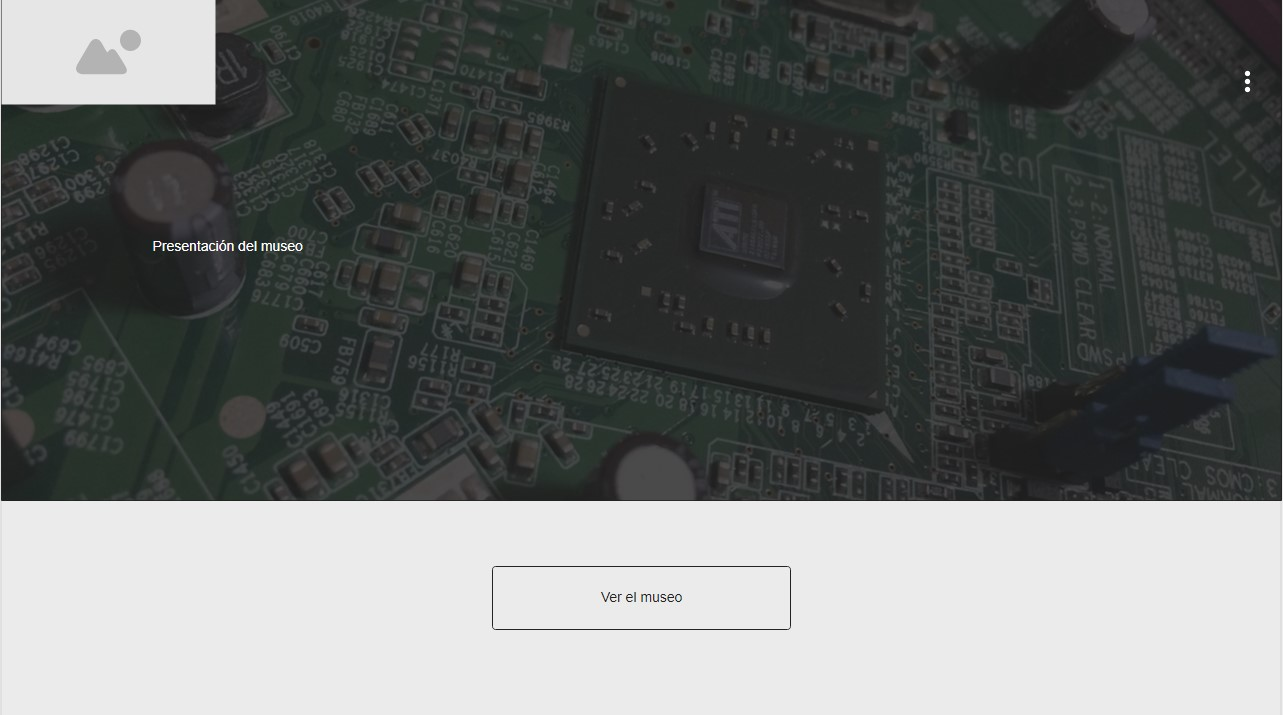
\includegraphics[scale=0.45]{homeIU}
\caption{Prototipo: Página de inicio}
\end{figure}
\paragraph*{Vista general del museo}
En la vista general del museo encontramos un menú lateral con filtros de búsqueda, y una sección principal que contiene una línea temporal con los periodos en los que se divide la historia de las CPUs.
\begin{figure}[H]
\centering
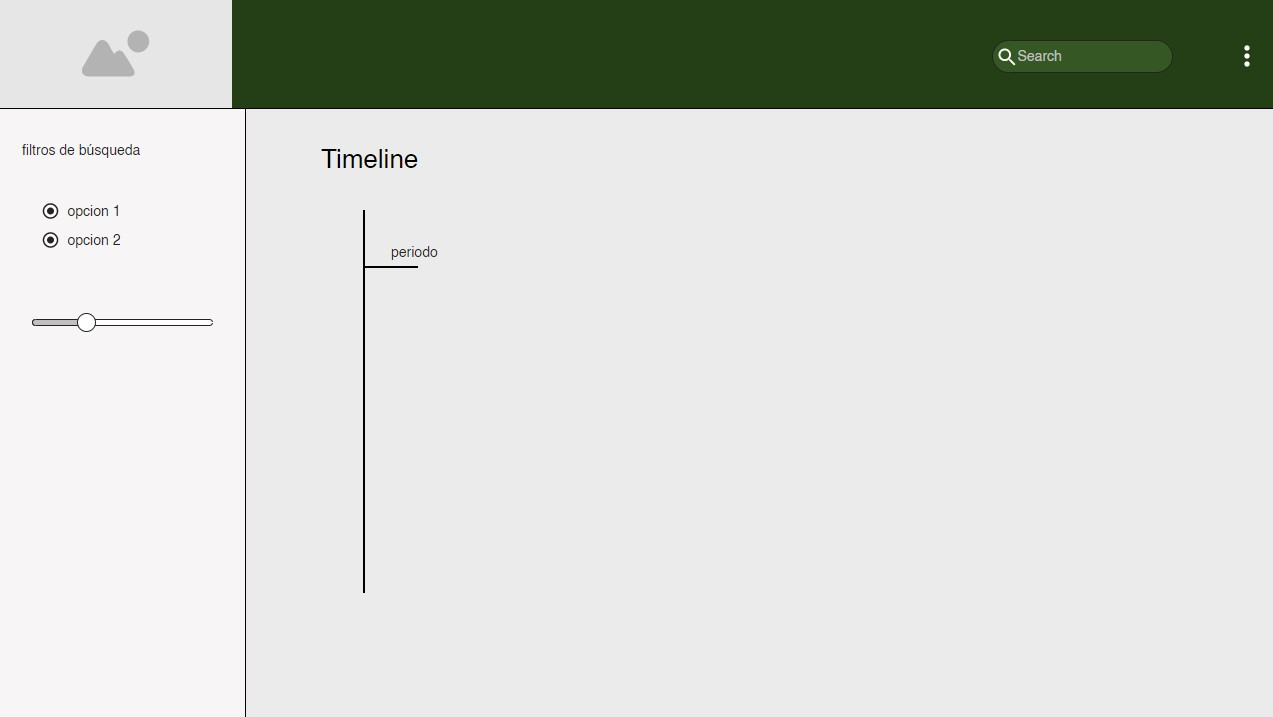
\includegraphics[scale=0.45]{museoIU}
\caption{Prototipo: Página de la vista general del museo}\label{iu:timeline}
\end{figure}
\paragraph*{Detalles del periodo}
En esta página hay un menú para volver a la vista general, y se muestran todos los detalles de un periodo (nombre, características, sistemas famosos de dicho periodo, etc.) y los componentes que pertenecen al mismo. 
\begin{figure}[H]
\centering
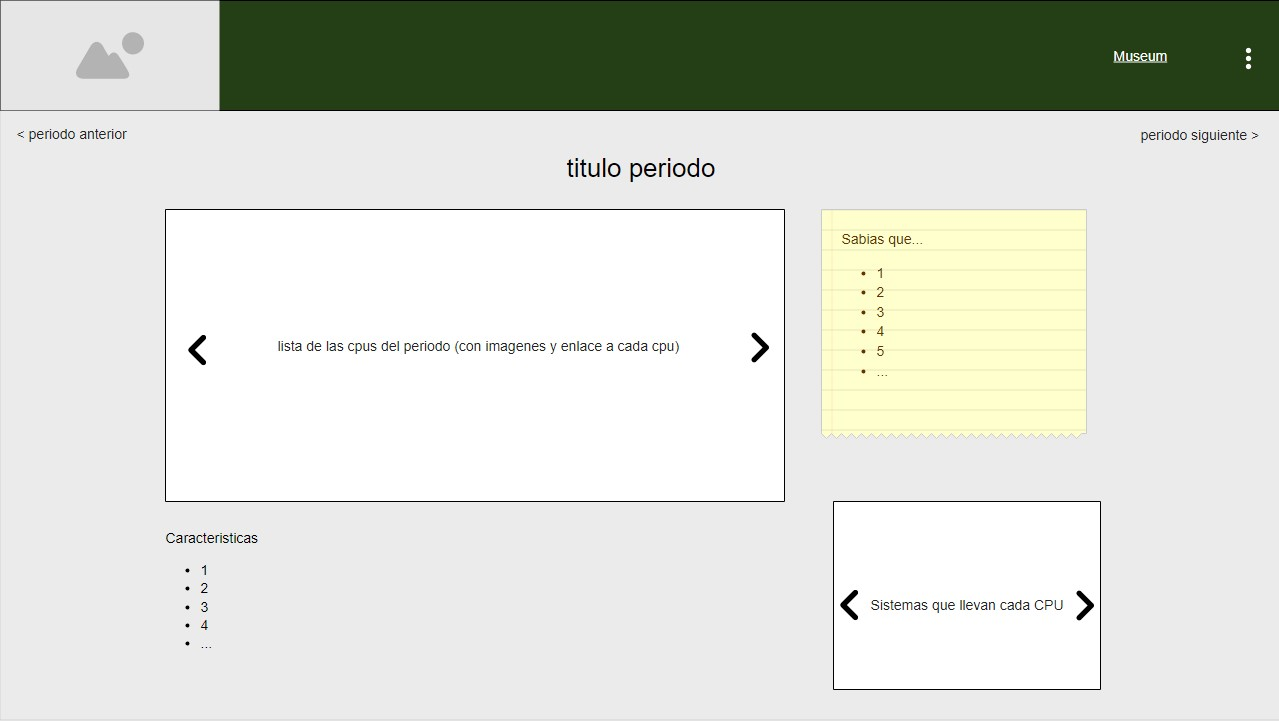
\includegraphics[scale=0.45]{periodoIU}
\caption{Prototipo: Página de detalles del periodo (museo)}\label{iu:period-details}
\end{figure}
\paragraph*{Detalles del componente}
En esta página se muestra una galería de fotos del componente, la descripción del mismo, y un listado de características. En el menú de esta página hay un listado de componentes pertenecientes al mismo periodo.
\begin{figure}[H]
\centering
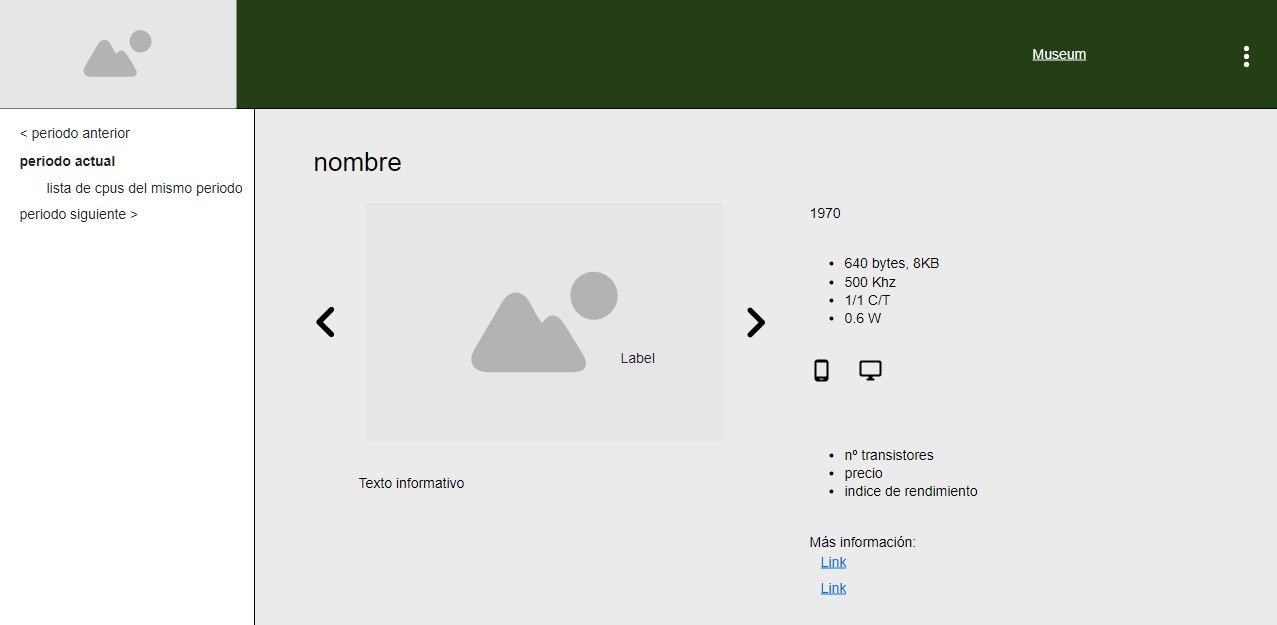
\includegraphics[scale=0.45]{piezaIU}
\caption{Prototipo: Página de detalles del componente (museo)}\label{iu:comp-details}
\end{figure}

\subsubsection{Administración del museo}
A continuación, se muestran los prototipos inciales para la aplicación de administración del museo. En todas ellas, salvo en la de inicio de sesión, hay un menú lateral de navegación. 
\paragraph*{Iniciar sesión}
En esta página el administrador del sistema deberá introducir su usuario y contraseña para acceder al mismo.
\begin{figure}[H]
\centering
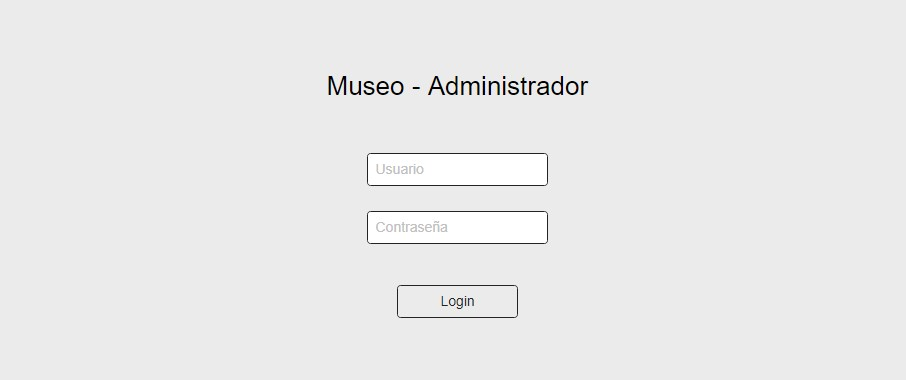
\includegraphics[scale=0.55]{loginIU}
\caption{Prototipo: Página de inicio de sesión}\label{iu:login}
\end{figure}
\paragraph*{Listado de periodos}
En esta página se muestra un listado de los periodos existentes, con las opciones de acceder a cada uno, editarlo o eliminarlo.
\begin{figure}[H]
\centering
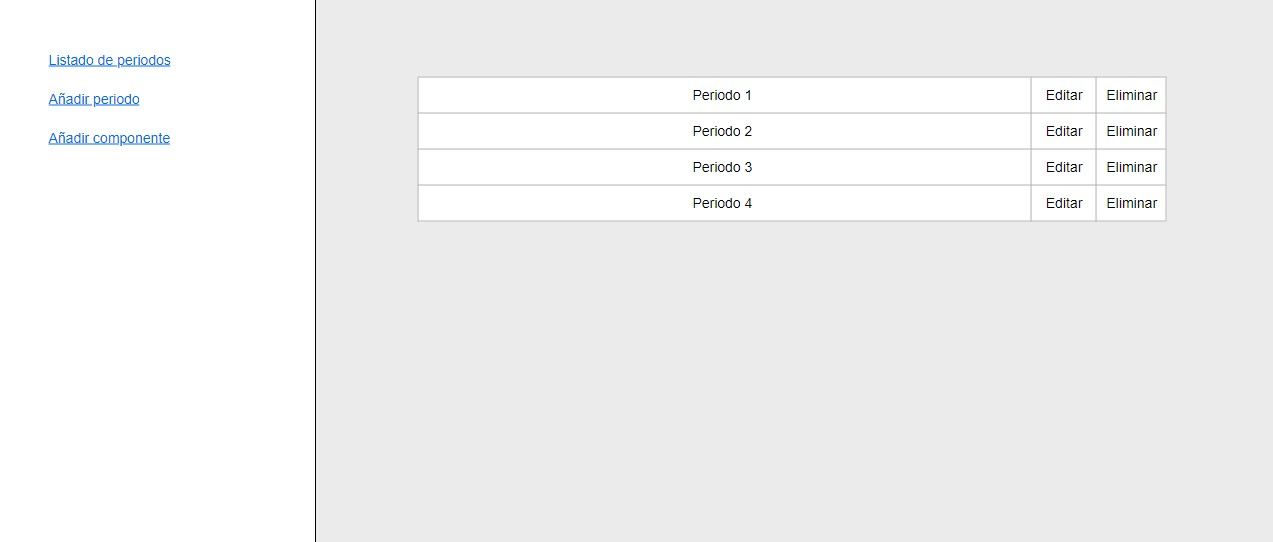
\includegraphics[scale=0.45]{listadoPeriodosIU}
\caption{Prototipo: Página de listado de periodos}\label{iu:list-periods}
\end{figure}
\paragraph*{Periodo}
Esta página contiene los detalles de un periodo así como un listado de los componentes pertenecientes al mismo, ofreciendo la opción de acceder a ellos, editarlos o eliminarlos.
\begin{figure}[H]
\centering
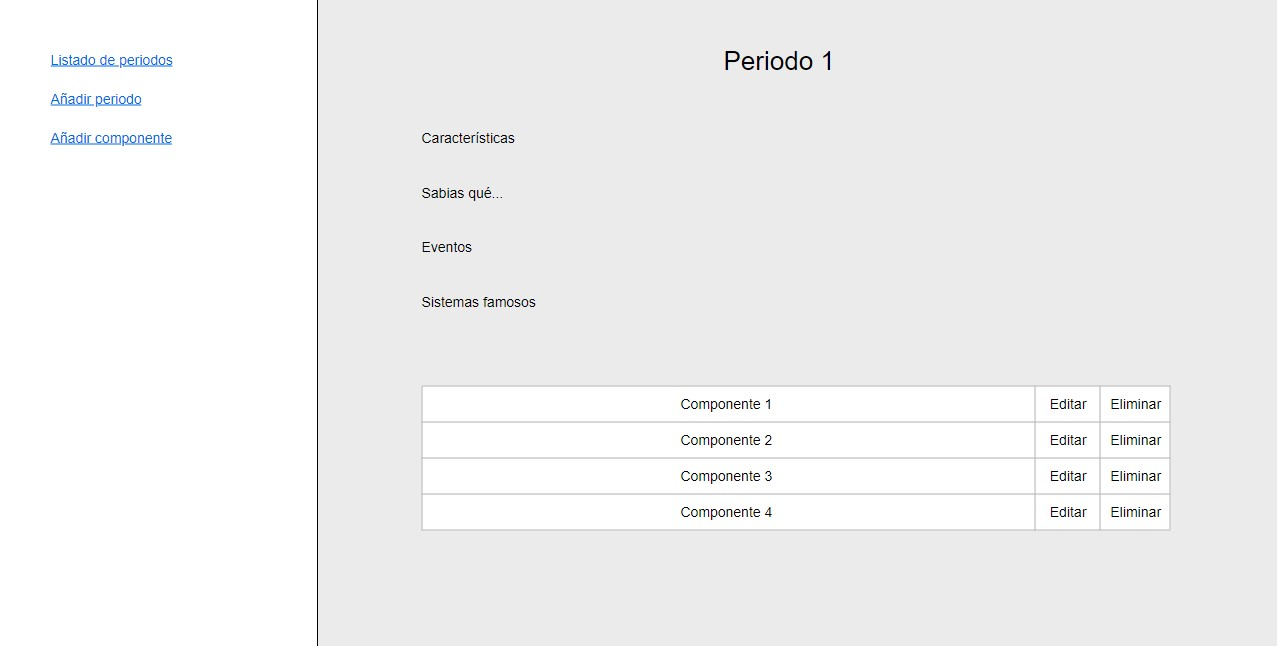
\includegraphics[scale=0.45]{periodoIU2}
\caption{Prototipo: Página de detalles de un periodo (admimnistración)}\label{iu:period}
\end{figure}
\paragraph*{Componente}
En esta página se muestran los detalles correspondientes al componente.
\begin{figure}[H]
\centering
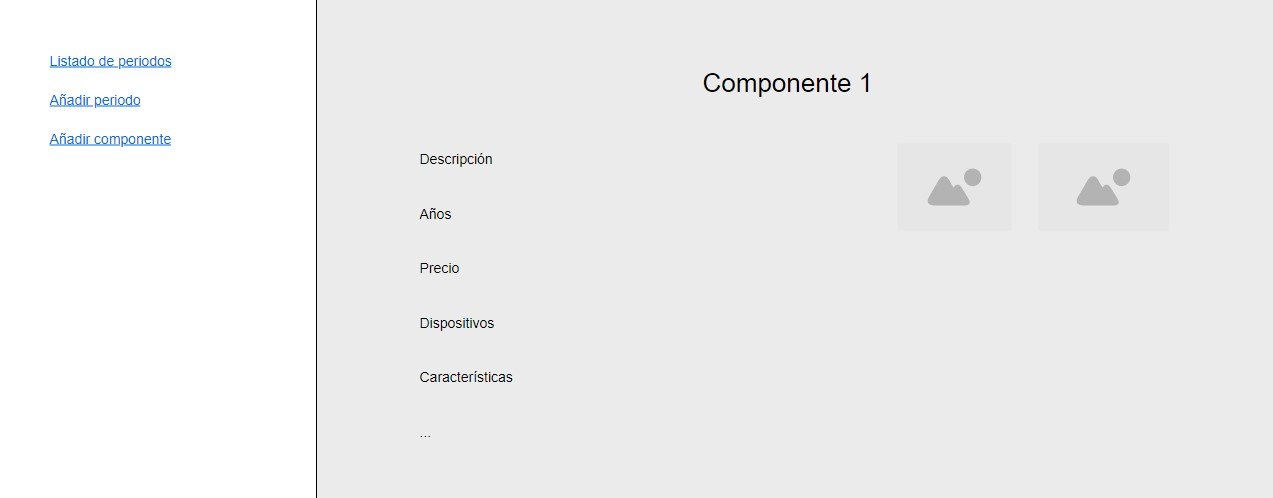
\includegraphics[scale=0.45]{compIU}
\caption{Prototipo: Página de detalles de un componente (admimnistración)}\label{iu:my-comp}
\end{figure}
\paragraph*{Añadir/editar periodo}
Los formularios para añadir o editar un periodo son idénticos, con la única diferencia de que el formulario para editar ya tiene los campos completados con los valores existentes del periodo, por tanto solo se muestra una captura representando ambos.
\begin{figure}[H]
\centering
\includegraphics[scale=0.45]{añadirPeriodoIU}
\caption{Prototipo: Formulario para añadir o editar un periodo}\label{iu:add-period}
\end{figure}
\paragraph*{Añadir/editar componente}
Con los formularios para añadir o editar un componente ocurre igual que con los del periodo ya mencionados.
\begin{figure}[H]
\centering
\includegraphics[scale=0.45]{añadirCompIU}
\caption{Prototipo: Formulario para añadir o editar un componente}\label{iu:add-comp}
\end{figure}



%\subsection{Descripción del Comportamiento de la Interfaz} 

\subsection{Diagrama de Navegabilidad}
A continuación se presentan dos diagramas de navegabilidad, correspondientes a las dos aplicaciones web que constituyen el sistema.
\subsubsection{Museo}
\begin{figure}[H]
\centering
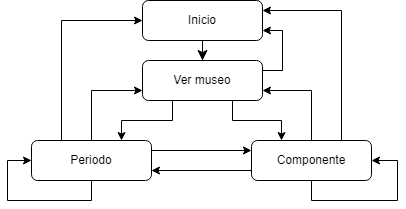
\includegraphics[scale=0.7]{nav-museo}
\caption{Diagrama de navegabilidad del museo}
\end{figure}

\subsubsection{Administración del museo}
\begin{figure}[H]
\centering
\centerline{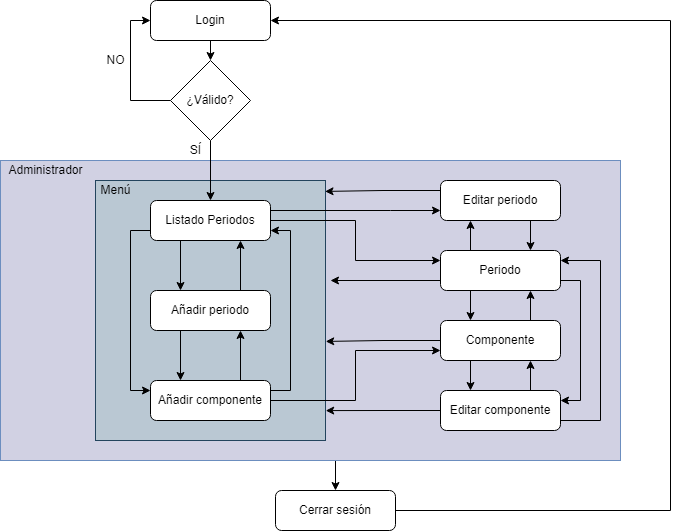
\includegraphics[scale=0.7]{nav-admin}}
\caption{Diagrama de navegabilidad de la administración del museo}
\end{figure}


\newpage
\section{ASI 10: ESPECIFICACIÓN DEL PLAN DE PRUEBAS}

\subsection{Pruebas unitarias}
Se realizarán pruebas unitarias del sistema utilizando Jasmine y Karma, herramientas incluidas en Angular para probar el correcto funcionamiento de los diferentes componentes.
\begin{table}[H]
%\vspace{-4mm}
  \centering
  \caption{Pruebas unitarias: Caso de uso 1}
    \begin{tabular}{p{9em}p{27em}}
    \toprule
    \rowcolor[rgb]{ .851,  .886,  .953} \multicolumn{2}{p{36em}}{\textbf{Caso de uso 1: Consultar periodos (museo)}} \\ \midrule
    \rowcolor[rgb]{ .949,  .949,  .949} \textbf{Prueba} &  \textbf{Resultado esperado}\\ \midrule
    \textbf{Obtener periodos existentes} & El sistema devolverá una lista de todos los periodos existentes. \\ \midrule
    \textbf{Obtener periodo por nombre} & El sistema devolverá una lista de los periodos cuyo nombre contenga el texto introducido. \\ \midrule
    \textbf{Obtener periodo por años} & El sistema devolverá una lista de los periodos cuyos años coincidan con los introducidos.\\ \bottomrule
    \end{tabular}%
\end{table}%
\begin{table}[H]
\vspace{-4mm}
  \centering
  \caption{Pruebas unitarias: Caso de uso 2}
    \begin{tabular}{p{11em}p{25em}}
    \toprule
    \rowcolor[rgb]{ .851,  .886,  .953} \multicolumn{2}{p{36em}}{\textbf{Caso de uso 2: Consultar componentes (museo)}} \\ \midrule
    \rowcolor[rgb]{ .949,  .949,  .949} \textbf{Prueba} &  \textbf{Resultado esperado}\\ \midrule
    \textbf{Obtener componentes de un periodo} & El sistema devolverá una lista de todos los componentes pertenecientes al periodo. \\ \bottomrule
    \end{tabular}%
\end{table}%
\begin{table}[H]
\vspace{-4mm}
  \centering
  \caption{Pruebas unitarias: Caso de uso 3}
    \begin{tabular}{p{9em}p{27em}}
    \toprule
    \rowcolor[rgb]{ .851,  .886,  .953} \multicolumn{2}{p{36em}}{\textbf{Caso de uso 3: Iniciar sesión}} \\ \midrule
    \rowcolor[rgb]{ .949,  .949,  .949} \textbf{Prueba} &  \textbf{Resultado esperado}\\ \midrule
    \textbf{Iniciar sesión con datos válidos } & El sistema permitirá el acceso a la página de administración. \\ \midrule
    \textbf{Iniciar sesión con datos incorrectos} & El sistema no permitirá el acceso y se mostrará un error. \\ \bottomrule
    \end{tabular}%
\end{table}%
\begin{table}[H]
\vspace{-4mm}
  \centering
  \caption{Pruebas unitarias: Caso de uso 4}
    \begin{tabular}{p{9em}p{27em}}
    \toprule
    \rowcolor[rgb]{ .851,  .886,  .953} \multicolumn{2}{p{36em}}{\textbf{Caso de uso 4: Consultar periodos (administración)}} \\ \midrule
    \rowcolor[rgb]{ .949,  .949,  .949} \textbf{Prueba} &  \textbf{Resultado esperado}\\ \midrule
    \textbf{Obtener periodos existentes} & El sistema devolverá una lista de todos los periodos existentes. \\ \bottomrule
    \end{tabular}%
\end{table}%
\begin{table}[H]
\vspace{-4mm}
  \centering
  \caption{Pruebas unitarias: Caso de uso 5}
    \begin{tabular}{p{11em}p{25em}}
    \toprule
    \rowcolor[rgb]{ .851,  .886,  .953} \multicolumn{2}{p{36em}}{\textbf{Caso de uso 5: Añadir periodo}} \\ \midrule
    \rowcolor[rgb]{ .949,  .949,  .949} \textbf{Prueba} &  \textbf{Resultado esperado}\\ \midrule
    \textbf{Añadir nuevo periodo} & El sistema tendrá un periodo más. \\ \midrule
    \textbf{Añadir periodo que ya existe} & El sistema no añadirá el periodo y responderá con un error.  \\ \midrule
    \textbf{Añadir periodo con campos vacíos} & El sistema no añadirá el periodo y responderá con un error. \\ \bottomrule
    \end{tabular}%
\end{table}%
\begin{table}[H]
\vspace{-4mm}
  \centering
  \caption{Pruebas unitarias: Caso de uso 6}
    \begin{tabular}{p{11em}p{25em}}
    \toprule
    \rowcolor[rgb]{ .851,  .886,  .953} \multicolumn{2}{p{36em}}{\textbf{Caso de uso 6: Modificar periodo}} \\ \midrule
    \rowcolor[rgb]{ .949,  .949,  .949} \textbf{Prueba} &  \textbf{Resultado esperado}\\ \midrule
    \textbf{Modificar periodo existente} & El sistema actualizará los datos del periodo. \\ \midrule
    \textbf{Modificar un periodo que no existe} & El sistema responderá con un error. \\ \midrule
    \textbf{Modificar periodo dejando campos vacíos} & El sistema no actualizará el periodo y responderá con un error. \\ \bottomrule
    \end{tabular}%
\end{table}%
\begin{table}[H]
\vspace{-4mm}
  \centering
  \caption{Pruebas unitarias: Caso de uso 7}
    \begin{tabular}{p{11em}p{25em}}
    \toprule
    \rowcolor[rgb]{ .851,  .886,  .953} \multicolumn{2}{p{36em}}{\textbf{Caso de uso 7: Eliminar periodo}} \\ \midrule
    \rowcolor[rgb]{ .949,  .949,  .949} \textbf{Prueba} &  \textbf{Resultado esperado}\\ \midrule
    \textbf{Eliminar un periodo existente} & El sistema tendrá un periodo menos. \\ \midrule
    \textbf{Eliminar un periodo que no existe} & El sistema responderá con un error. \\ \bottomrule
    \end{tabular}%
\end{table}%
\begin{table}[H]
\vspace{-4mm}
  \centering
  \caption{Pruebas unitarias: Caso de uso 8}
    \begin{tabular}{p{11em}p{25em}}
    \toprule
    \rowcolor[rgb]{ .851,  .886,  .953} \multicolumn{2}{p{36em}}{\textbf{Caso de uso 8: Consultar componentes (administración)}} \\ \midrule
    \rowcolor[rgb]{ .949,  .949,  .949} \textbf{Prueba} &  \textbf{Resultado esperado}\\ \midrule
    \textbf{Obtener componentes de un periodo} & El sistema devolverá una lista de todos los componentes pertenecientes al periodo. \\ \bottomrule
    \end{tabular}%
\end{table}%
\begin{table}[H]
\vspace{-4mm}
  \centering
  \caption{Pruebas unitarias: Caso de uso 9}
    \begin{tabular}{p{13em}p{23em}}
    \toprule
    \rowcolor[rgb]{ .851,  .886,  .953} \multicolumn{2}{p{36em}}{\textbf{Caso de uso 9: Añadir componente}} \\ \midrule
    \rowcolor[rgb]{ .949,  .949,  .949} \textbf{Prueba} &  \textbf{Resultado esperado}\\ \midrule
    \textbf{Añadir nuevo componente} & El sistema tendrá un componente más. \\ \midrule
    \textbf{Añadir componente que ya existe} & El sistema no añadirá el componente y responderá con un error.  \\ \midrule
    \textbf{Añadir componente a un periodo que no existe} & El sistema no añadirá el componente y responderá con un error.  \\ \midrule
    \textbf{Añadir componente con campos obligatorios vacíos} & El sistema no añadirá el componente y responderá con un error. \\ \bottomrule
    \end{tabular}%
\end{table}%
\begin{table}[H]
\vspace{-4mm}
  \centering
  \caption{Pruebas unitarias: Caso de uso 10}
    \begin{tabular}{p{13em}p{23em}}
    \toprule
    \rowcolor[rgb]{ .851,  .886,  .953} \multicolumn{2}{p{36em}}{\textbf{Caso de uso 10: Modificar componente}} \\ \midrule
    \rowcolor[rgb]{ .949,  .949,  .949} \textbf{Prueba} &  \textbf{Resultado esperado}\\ \midrule
    \textbf{Modificar componente existente} & El sistema actualizará los datos del componente. \\ \midrule
    \textbf{Modificar un componente que no existe} & El sistema responderá con un error. \\ \midrule
    \textbf{Modificar componente dejando campos obligatorios vacíos} & El sistema no actualizará el componente y responderá con un error. \\ \bottomrule
    \end{tabular}%
\end{table}%
\begin{table}[H]
\vspace{-4mm}
  \centering
  \caption{Pruebas unitarias: Caso de uso 11}
    \begin{tabular}{p{13em}p{23em}}
    \toprule
    \rowcolor[rgb]{ .851,  .886,  .953} \multicolumn{2}{p{36em}}{\textbf{Caso de uso 11: Eliminar componente}} \\ \midrule
    \rowcolor[rgb]{ .949,  .949,  .949} \textbf{Prueba} &  \textbf{Resultado esperado}\\ \midrule
    \textbf{Eliminar un componente existente} & El sistema tendrá un componente menos. \\ \midrule
    \textbf{Eliminar un componente que no existe} & El sistema responderá con un error. \\ \bottomrule
    \end{tabular}%
\end{table}%

\subsection{Pruebas del sistema}\label{sec:pruebas-sistema}
Se probará el conjunto completo del sistema, es decir, si la aplicación, el servidor y la base de datos se conectan de forma correcta, sin errores en tiempo de ejecución y obteniendo las respuestas esperadas. Estas pruebas se realizarán de forma manual sobre la aplicación.
\subsection{Pruebas de usabilidad}
Para realizar estas pruebas se hará uso de una serie de cuestionarios, cuyos resultados se obtendrán tras observar como usuarios con diferentes perfiles interactúan con el sistema.


